%\documentclass{book}
\documentclass{article}                            %for shorter notes
\usepackage{graphicx}                              %for PNG images (pdflatex)
%\usepackage{graphics}                              %for EPS images (latex)
\usepackage[linkbordercolor={1.0 1.0 0.0}]{hyperref} %for \url tag
\usepackage{color}                                 %for defining custom colours
\usepackage{framed}                                %for shaded and framed paragraphs
\usepackage{textcomp}                              %for various symbols, e.g. Registered Mark
\usepackage{geometry}                              %for defining page size
\usepackage{longtable}                             %for breaking tables
%
\geometry{verbose,a4paper,tmargin=2.5cm,bmargin=2.5cm,lmargin=2.5cm,rmargin=2cm}
\hypersetup{
  pdfauthor = {Author Name},
  pdftitle = {Paper title},
  pdfsubject = {Paper subject},
  pdfkeywords = {Paper,keyword,comma-separated},
  pdfcreator = {PDFLaTeX with hyperref package},
  pdfproducer = {PDFLaTeX}
}
%
\bibliographystyle{IEEEtran}                       %a nice bibliography style
%
\def\efill{\hfill\nopagebreak}%
\hyphenation{Nordu-Grid}
\setlength{\parindent}{0cm}
\setlength{\FrameRule}{1pt}
\setlength{\FrameSep}{8pt}
\addtolength{\parskip}{5pt}
\renewcommand{\thefootnote}{\fnsymbol{footnote}}
\renewcommand{\arraystretch}{1.3}
\newcommand{\dothis}{\colorbox{shadecolor}}
\newcommand{\globus}{Globus Toolkit\textsuperscript{\textregistered}~2~}
\newcommand{\GT}{Globus Toolkit\textsuperscript{\textregistered}}
\newcommand{\ngdl}{\url{http://ftp.nordugrid.org/download}~}
\definecolor{shadecolor}{rgb}{1,1,0.6}
\definecolor{salmon}{rgb}{1,0.9,1}
\definecolor{bordeaux}{rgb}{0.75,0.,0.}
\definecolor{cyan}{rgb}{0,1,1}
%
%----- DON'T CHANGE HEADER MATTER
\begin{document}
\def\today{\number\day/\number\month/\number\year}

\begin{titlepage}

\begin{tabular}{rl}
\resizebox*{3cm}{!}{
\includegraphics{ng-logo.png}}
&\parbox[b]{2cm}{\textbf \it {\hspace*{-1.5cm}NORDUGRID\vspace*{0.5cm}}}
\end{tabular}

\hrulefill

%-------- Change this to NORDUGRID-TECH-NN

{\raggedleft NORDUGRID-TECH-NN\par}

{\raggedleft \today\par}

\vspace*{2cm}

%%%%---- The title ----
{\centering \textsc{\Large ARC Accounting Component -- JURA}\Large \par}
\vspace*{0.5cm}
    
%%%%---- A subtitle, if necessary ----
{\centering \textit{\large Technical document}\large \par}
    
\vspace*{1.5cm}
%%%%---- A list of authors ----
    {\centering \large P\'eter D\'ob\'e \footnote{dobe@iit.bme.hu} \large \par}
    
%%%%---- An abstract - if style is article ----
%\begin{abstract}
%The abstract
%\end{abstract}
\end{titlepage}

%\tableofcontents                          %Comment if use article style
\newpage

\section{Purpose}

The \textit{Job Usage Reporter of ARC} (JURA) is a component
implementing accounting functionality in the ARC middleware. Its
objective is to gather metered resource usage data for each job and
submit it to accounting services along with the job submitter's
identity and miscellaneous job-related metadata.

The accounting service stores the received usage data in a database,
and provides an interface for querying it. Queries can be made by the
consumers of the accounting data, such as a billing component. The
service itself is a third party application, separate from the
middleware distribution. JURA is currently capable of using the
logging service of the SweGrid Accounting System (SGAS)\cite{sgas},
but maintaining the possibility to enable utilising other services has
been kept in mind during design.

Before the usage data collected from the resource manager is
submitted, it is transformed into records of job-level granularity. To
every job corresponds exactly one Grid user, therefore reports over a
time period (e.g.~an invoice) can be generated per-user, or
alternatively on a larger scale such as job project or VO level.

\section{Architecture}

\begin{figure}[ht]
\centering{{{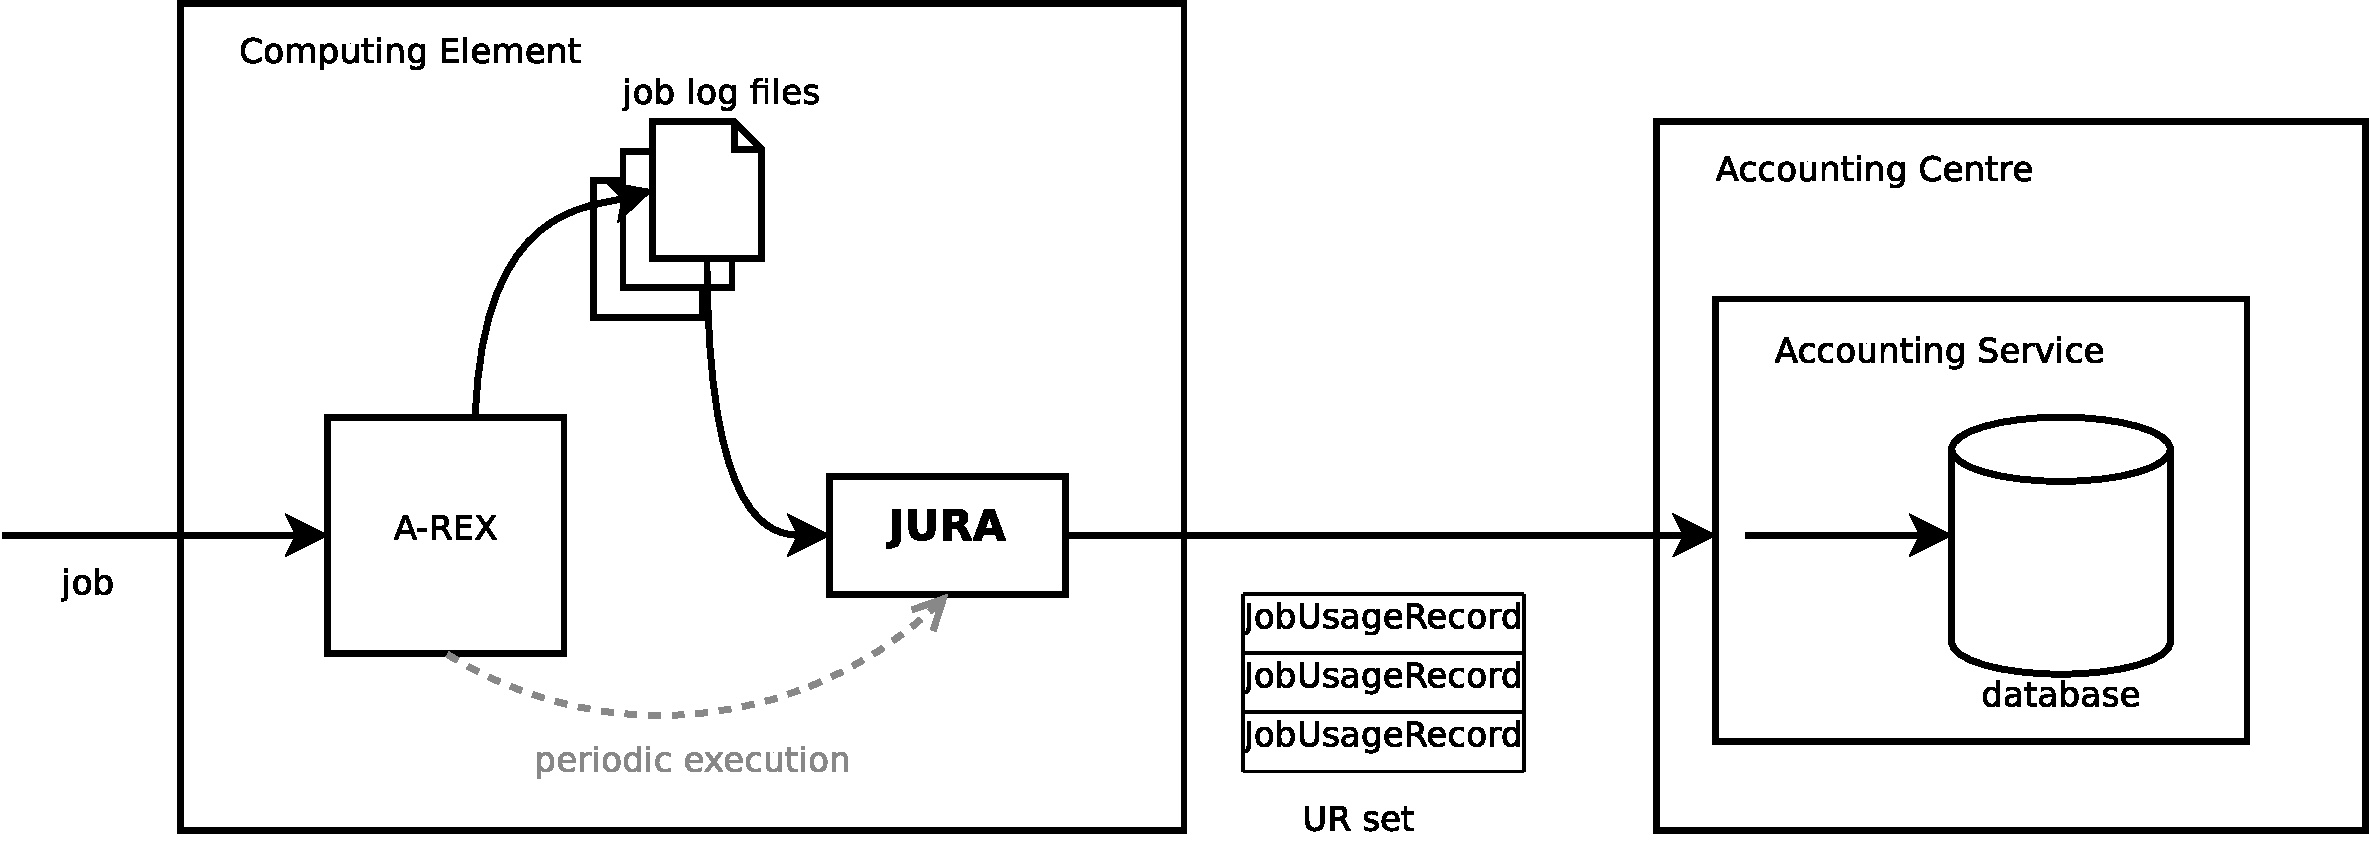
\includegraphics[width=0.9\textwidth]{components.pdf}}}
\caption{\label{fig:components}Components participating in accounting.} }
\end{figure}

JURA offers a complete replacement in functionality for the old
\textit{logger} utility\cite{logger}, a job metadata logging tool with
a purpose very closely related to that of this new tool. However,
backwards compatibility is maintained, so the old logger can still be
deployed.

The ARC execution manager, A-REX\cite{arex} initiates JURA in a
similar way to invoking logger. JURA reads job log files provided by
A-REX. These files have the same format as those meant for logger,
with additional lines which are necessary for accounting scenarios.

It also acts as a client for one or more accounting services,
specifically SGAS Logging and Usage Tracking Services (LUTS's),
inserting the generated records in batches. (See Figure
\ref{fig:components}.)

\section{Operation}

\subsection{Invocation}

JURA is a stand-alone executable application, executed hourly by
A-REX. It has no separate configuration file; it gets all necessary
configuration options from A-REX, in part through command-line
arguments, but mostly via lines in the job log files (see Appendix
\ref{config} for details). The source of the latter are lines in the
grid-manager configuration file.

The command line format is a subset of that of logger:

\verb|jura [-E <expiration_time>] <control_dir>|

where \textit{expiration\_time} is the validity length of job log
files in days, after which time they are considered invalid;
\textit{control\_dir} is the A-REX control directory for a mapped
local UNIX user.

\subsection{Parsing job log files}
\label{joblogs}
The job log files generated by A-REX reside under the directory
\textit{<control\_dir>/logs}. They have file name format
\textit{<ngjobid>.<random>}, where \textit{ngjobid} is the identifier
created for the job by A-REX, \textit{random} is a randomly generated
sequence of alphanumeric characters to avoid collision of different
files pertaining to the same job. For each job and for each reporting
destination (i.e. accounting service to be contacted), at least two
log files are written for each job: one at the time of job submission,
and another one after the job finishes, and possibly others at each
start and stop event.

A job log file consists of ``\textit{name=value}'' lines.  These
make up some of the configuration options for JURA, such as the URL of
an accounting destination in the ``\textit{loggerurl=}'' line.  The
file also contains detailed resource usage data and related metadata
to be reported about the job.(See Appendix \ref{config} for more
details.)  The accuracy of the metered data may depend on the type of
batch system used.

Based on the usage data in the processed job log file, JURA assembles
records in the format proposed by the Open Grid Forum (OGF), called
the \textit{Usage Record} (UR)\cite{ur}. This is an XML representation
holding consumption information for all commonly used resources and
metrics. It can be extended by custom elements for non-standard
resources and/or other types of job metadata. For a list of UR
properties used by JURA, see Appendix \ref{log2ur}.

Some elements of UR are mandatory, these must all be present in the
job log file to be able to generate a UR. For example, the job log
file generated upon job submission contains no \textit{status} entry,
so this file is ignored, and no UR is generated from it.

\subsection{Accessing LUTS}
After the necessary URs to be inserted are filled and valid, they are
submitted to the accounting service through its insertion
interface. The service in particular, SGAS LUTS has a simple custom
web service interface loosely based on WS-ResourceProperties.

To increase communication efficiency, LUTS accepts a batch of several
URs within a single request. The batch is an XML element called
\textit{UsageRecords}, containing elements representing URs. The
maximal number of URs in a batch is limited, it can be set in the
``\textit{jobreport\_options=}'' line of the A-REX configuration file
(see Appendix \ref{config}).

\section{Security}
The JURA executable runs as the same user as A-REX does, typically as
\textit{root}. The owner of a job log file is the local user mapped
for the submitter entity of the corresponding job. These files contain
confidential data, access to which must be restricted, therefore read
access is limited to the owner and the super user. If JURA is executed
by A-REX, it can read data from these files, and delete expired files.

The authentication towards the SGAS LUTS is done via the standard
X.509 certificate mechanism over SSL protocol: a chain of valid
(i.e. not expired and/or revoked) certificates with a trusted root
certification authority is accepted as authentic identification of the
client. This means that the client can access the service using a
proxy certificate as well. In the scenario involving A-REX and JURA,
all usage records are submitted using credentials given in the
\textit{jobreport\_credentials} line of the A-REX configuration file
(see Appendix \ref{config}), and no proxies are used. Normally the
credentials for the A-REX service should be used.

The access control policy for LUTS can be configured in two ways. One
is a plain text configuration file where users, identified by their
DNs, can be granted or denied publish and/or query rights for all
URs. The other option is a service port type called \textit{Service
  Authorization Management} (SAM). One can set access control rules
through the SAM port of the service in a format based on XACML. 

\section{Implementation}
JURA is written merely in C++, and is tested in a GNU/Linux
environment, built with standard GNU tools. It depends on the HED
libraries, and thus also on all mandatory dependencies thereof. The
\textit{openssl} library is also required, since sensitive accounting
data needs to be sent in a secure manner.

%TODO about other service types

When deployed, the executable called ``\textit{jura}'' is placed into the
\textit{libexec} directory of the ARC install location. There is a
symbolic link %TODO make it so!
to the executable in the same directory, called ``\textit{logger}'',
through which A-REX executes JURA. This is to keep compatibility with
the old logger client. No other executables or wrapper scripts are
needed.

\appendix

\section{Configuration}
\label{config}

%   loggerurl: jobreport, JSDL

%   (lifetime)

%   jobreport

%   accounting\_options: jobreport\_options

%   key\_path, certificate\_path, ca\_certificates\_dir: jobreport\_credentials

\section{Usage Record properties}
\label{log2ur}
%   input file format

%   filled properties

%   missing properties

\bibliography{grid}
\end{document}
